\documentclass[../main.tex]{subfiles}

\begin{document}

\newcommand{\flippedstep}[3]{
    \begin{tcolorbox}[
        boxrule=0pt, colframe=black!5,
        coltitle=black, colback=#1,
        step=sample,
        height=7.5cm
    ]
    \begin{center}
        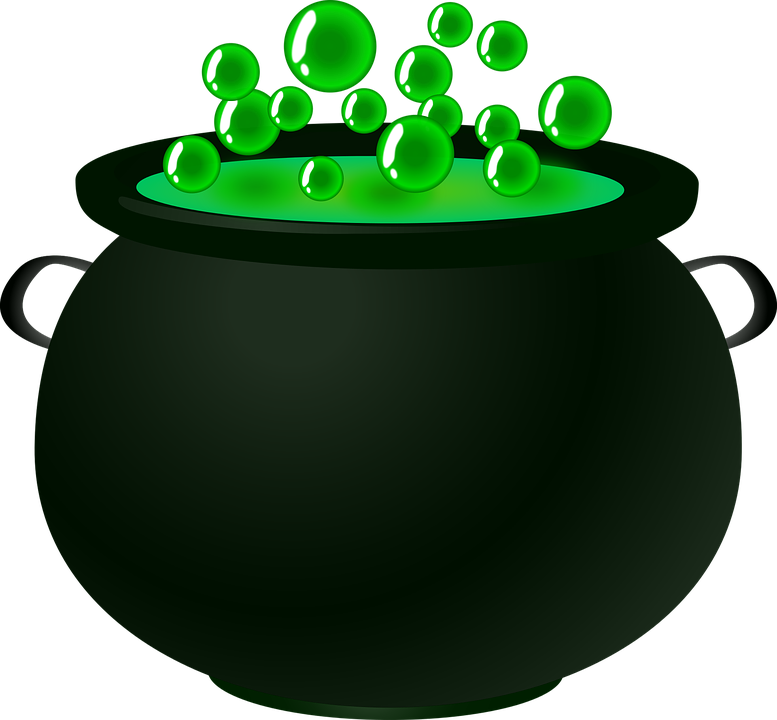
\includegraphics[height=3cm]{images/zaubertrank.png}
    \end{center}
    \tcblower
    \begin{center}
        \textbf{#2}
    \end{center}
    \scriptsize #3
    \end{tcolorbox}
}
\parpic[r]{
    \tikz[scale=1.9]{\sloth}
}
Bevor es mit der Mathematik losgeht, möchten wir gern noch ein paar Worte darüber verlieren, wie das Lernen mit diesem Buch und den Begleitmaterialien, die dafür erstellt worden sind, gedacht ist. Wir möchten außerdem das Lehrkonzept \emph{Flipped Classroom} genauer erläutern, damit du das beste für dich dabei herausholen kannst. Um dir nur das zu erklären, was für dich interessant ist, haben wir diese Einführung danach unterteilt, wer du bist und was deine Ziele sind, wenn du mit diesem Buch arbeitest. Wir gehen davon aus, dass auf dich einer der folgenden Punkte zutrifft.

\begin{enumerate}
    \item Du bist \textbf{Schüler} und dein Lehrer hat sich entschieden, dieses Buch für seinen Matheunterricht zu verwenden.
    \item Du bist \textbf{Lehrer} und möchtest unser Buch bei deiner Unterrichtsgestaltung verwenden.
    \item Du bist einfach so auf dieses Buch gestoßen und möchtest deine mathematischen Grundlagen festigen oder vertiefen.
\end{enumerate}

Auf den nächsten Seiten stellen wir dir unser Buch und die dazugehörigen Materialien vor und erklären dir, wie du damit möglichst sinnvoll arbeiten kannst. Wir haben diese Erklärungen danach aufgeteilt, das dich vermutlich interessiert -- abhängig davon, ob du ein Lehrer, ein Schüler oder nichts von beidem bist.

Wenn du ein \textbf{Schüler} bist, dann gehen wir davon aus, dass dein Lehrer sich dafür entschieden hat, mit dem Reiseführer ein \emph{Flipped Classroom}-Konzept umzusetzen. Bist du dir nicht sicher, dann frage nochmal nach. Was das \emph{Flipped Classroom}-Konzept ist und wie du damit arbeiten kannst, erklären wir dir im Abschnitt \enquote{Lernen mit Flipped Classroom}. Den Abschnitt zum Aufbau dieses Buchs kannst du überspringen, da er für diejenigen gedacht ist, die mit diesem Buch lernen wollen, aber kein Flipped Classroom-Konzept verwenden.

Falls du ein \textbf{Lehrer} bist, empfehlen wir dir, alles durchzulesen, damit du die verschiedenen Arbeitsweisen, die wir empfehlen, kennst und dich auf sie einstellen kannst. Extra für Lehrer gibt es außerdem noch einen Abschnitt \enquote{Unterrichtsgestaltung mit dem Reiseführer Mathematik}. In diesem erklären wir dir, wie du den Reiseführer Mathematik für einen gelungenen Unterricht verwenden kannst und welche Möglichkeiten du hast, ihn an die Inhalte, die du vermitteln möchtest, anzupassen. Wir stellen dir dort außerdem weitere Ideen vor, die wir im Zusammenhang mit diesem Lehrmaterial erarbeitet haben.

Wenn du das Buch als Nachschlagewerk oder zum Nacharbeiten von Schulwissen verwendest, interessiert dich vermutlich vor allem der \emph{Aufbau dieses Buchs} (also der nächste Abschnitt). Dort stellen wir die verschiedenen Komponenten des Reiseführers Mathematik vor und geben dir eine grobe Idee davon, wie du sie verwenden kannst.

\newpage
\section*{Aufbau dieses Buchs}
\label{concept}

Zum \emph{Reiseführer Mathematik} gehört nicht nur dieses Buch, sondern noch eine Reihe weiterer Materialien. Insgesamt besteht dieses Lehrwerk aus den folgenden Komponenten:
\begin{enumerate}
    \item diesem \textbf{Buch}, das Erklärungen zu den üblicherweise in der Schule behandelten Themen enthält
    \item pro Kapitel einem Satz \textbf{Vorbereitungsblätter}, die jeweils den Abschnitten dieses Buchs zugeordnet sind und eine Hilfestellung beim Durcharbeiten der entsprechenden Abschnitte sein sollen
    \item pro Kapitel einem \textbf{Aufgabenblock}, der Übungsaufgaben verschiedener Schwierigkeitsgrade sowie Beispiellösungen zu den Inhalten des entsprechenden Kapitels enthält
    \item \textbf{Erklärvideos}, die dieselben Inhalte wie das Buch behandeln
\end{enumerate}

Dieses Buch unterscheidet sich von den meisten Lehrbüchern, weil es keine Aufgaben enthält. Stattdessen kannst du in diesem Buch viele Beispiele und ausführlichere Erklärungen finden.

Jedes Kapitel in diesem Buch ist in verschiedene Abschnitte aufgeteilt (z.\,B. die Einführung). In diesen Abschnitten erklären wir dir das gerade behandelte Thema so, dass du es (ggf. mit dem Vorwissen aus den vorangegangenen Kapiteln) verstehen kannst. Dabei verwenden wir viele ausführliche Beispiele und Erklärungen. Du musst dir nicht unbedingt alle Beispiele genau durchlesen, wenn du dir zutraust, das Thema auch ohne sie zu verstehen. Alle Inhalte, die wichtig sind, werden im Text außerhalb der Beispiele so erklärt, dass du auch ohne die Beispiele verstehen kannst, worum es geht. 

\begin{example}{}
    Wenn wir versuchen, dir zu erklären, dass die Regel \emph{Punkt- vor Strichrechnung} gilt, dann schreiben wir dies im Text außerhalb des Beispiels. Vielleicht verstehst du direkt, was gemeint ist, aber möglicherweise hilft es dir auch, ein Beispiel durchzulesen, in dem wir dir am konkreten Beispiel $6+9\cdot 3$ zeigen, dass du erst $9\cdot 3$ rechnen musst und nicht zuerst $6+9$.
\end{example}

Um dir später das Wiederholen der Inhalte zu erleichtern, endet jeder Abschnitt mit einer Zusammenfassungsbox wie der folgenden.

\begin{nutshell}{Zusammenfassungsboxen}
    Am Ende jedes Abschnitts in diesem Buch findest du eine Box wie diese. Hier werden alle wichtigen Erkenntnisse, die im Abschnitt vorkamen, genannt und knapp erklärt. Eine Zusammenfassungsbox enthält jedoch keine ausführlichen Erklärungen oder Beispiele. Mithilfe dieser Boxen kannst du einen guten Überblick über die Themen bekommen, wenn du sie bereits verstanden hast.
\end{nutshell}

\begin{advanced}{Weiterführendes Wissen}
    Zusätzlich zu den Inhalten, die für die Schulmathematik zwingend notwendig sind, enthält dieses Buch auch Einblicke in Themen, die darüber hinaus gehen. Falls die normalen Themen keine ausreichende Herausforderung für dich sind und du dich mit ein wenig komplizierteren Themen beschäftigen möchtest, dann solltest du nach den violett hinterlegten Teilen im Buch Ausschau halten. Diese befinden sich zum einen am Ende jedes Kapitels. Darüber hinaus findest du hin und wieder violett hinterlegte Blöcke wie diesen, die über die Kapitel verteilt auftauchen. Sie enthalten Ergänzungen zu dem Thema, über das du gerade etwas gelesen hast und verweisen manchmal auf die violetten Seiten am Ende des Kapitels.

    Die Inhalte dieser Blöcke sind für das restliche Buch nicht weiter wichtig. Du wirst immer in der Lage sein, das Buch zu verstehen, auch wenn du diese Boxen einfach ignorierst, weil es im Buch keine Stellen gibt, die auf weiterführendem Wissen aufbauen.
\end{advanced}

Die beiden folgenden Kästen, die dir im Buch wie Sand am Meer begegnen werden, enthalten Informationen, die es besonders wert sind, sie sich zu merken. Besonders wichtige Erkenntnisse oder einfach nur Schreibweisen werden in diesen Kästen festgehalten.

\begin{definition}{}
    In Boxen wie dieser findest du Definitionen. Eine Definition ist eine Schreibweise oder ein Name, die sich Mathematiker für etwas ausgedacht haben, was sie häufig verwenden. Die neuen Begriffe, die wir in Definitionen einführen, machen uns das Leben einfacher, weil wir sie als eine Art Abkürzung für Dinge verwenden können, die wir sonst viel umständlicher aufschreiben müssten.
\end{definition}

\begin{theorem}{}
    Sätze sind eigentlich der spannendste Teil der Mathematik. Anders als Definitionen, in denen wir nur neue Schreibweisen einführen, ist ein Satz eine (hoffentlich interessante) Aussage, die immer gilt und die sich logisch aus dem, was wir bereits wissen, herleiten lässt. Wenn wir eine Erkenntnis in einem Satz festhalten, dann können wir später von dieser Erkenntnis profitieren und das Wissen aus dem Satz verwenden, wenn wir es brauchen.
\end{theorem}

Um dich beim Verstehen der Erklärungen aus dem Buch zu unterstützen, gibt es \textbf{Vorbereitungsblätter}. Jedes Vorbereitungsblatt gehört zu einem Abschnitt aus dem Buch (die Vorbereitungsblätter sind genauso nummeriert wie die Abschnitte in diesem Buch). Zu allen Abschnitten, die du im Inhaltsverzeichnis sehen kannst, gehört also ein Vorbereitungsblatt. Die einzige Ausnahme sind die Abschnitte mit weiterführendem Wissen, die im Buch violett hinterlegt sind und zu denen kein Vorbereitungsblatt gehört.

Ein Vorbereitungsblatt enthält alle wichtigen Definitionen und Sätze aus dem Abschnitt im Buch, zu dem es gehört. Die Buchstellen, die für ein Vorbereitungsblatt wichtig sind, findest du in den grauen Kästen auf den Vorbereitungsblättern. Auf der linken Seite dieser Kästen findest du außerdem immer einen QR-Code, der zu einem Video führt, das dieselben Inhalte erklärt. Du kannst dir also aussuchen, ob du die Inhalte lieber durch ein Video erklärt bekommen möchtest oder ob du sie dir lieber im Buch durchlesen möchtest.

\newtcolorbox{video}{code={\pgfkeysalsofrom{\tcmathenvopt}}, colback=black!10,colframe=black!30, boxsep=0pt}
\begin{video}
    \begin{minipage}{.1\textwidth}
        \qrcode[height=1cm]{https://themrsheldon.github.io/testing/}
    \end{minipage}
    \begin{minipage}{.9\textwidth}
        \href{https://themrsheldon.github.io/testing/}{\textbf{Video:} \textit{Beispiel-Video}} (5 Minuten)\\
        Aufbau dieses Buchs (ab Seite \pageref{concept})
    \end{minipage}
\end{video}

Du kannst ein Vorbereitungsblatt als eine Art Anleitung zum Durcharbeiten des Buchs verwenden. Es enthält eine Liste von Themen, die es dir beibringen möchte und durch die grauen Kästen Verweise auf unsere Erklärungen zu diesen Themen. Während du die Videos schaust oder die Seiten im Buch durchliest, auf die das Vorbereitungsblatt verweist, kannst du mit den Verständnisfragen auf dem Vorbereitungsblatt prüfen, ob du verstanden hast, was du gerade gelesen oder gehört hast. Zu jedem Video gehört deshalb ein kleiner Aufgabenteil mit Aufgaben, die du schnell durch das Ausfüllen eines Lückentextes, durch Ankreuzen oder ähnliches direkt auf dem Vorbereitungsblatt bearbeiten kannst.

Um das Thema eines Abschnitts in diesem Buch besser zu verstehen und zu üben, kannst du die Übungsaufgaben bearbeiten, die in den \textbf{Aufgabenblöcken}, die es zu jedem Kapitel gibt, enthalten sind. Die Übungsaufgaben ergänzen die Aufgaben auf dem Vorbereitungsblatt und erfodern meistens, dass du selbst etwas mehr aufschreibst. Sie unterteilen sich in verschiedene Schwierigkeitsstufen, die auf den Aufgabenblöcken genauer erklärt sind. Außerdem findest du auf den Aufgabenblöcken Beispiellösungen mit Erklärungen, die beschreiben, wie du an bestimmte Arten von Aufgaben herangehen kannst.

Falls du beim Bearbeiten von Aufgaben nicht weiterkommst, kannst du einen der Hinweise verwenden, die es zu den meisten Aufgaben aus den Aufgabenblocken gibt. Hinweise versuchen, dich in Richtung der Lösung zu lenken, ohne die Lösung dabei zu verraten. Schließlich endet jeder Aufgabenblock mit einem \textbf{Selbsttest}. Dieser besteht aus einer kleinen Sammlung von Aufgaben, die das gesamte Wissen des Kapitels voraussetzen und die du zum Beispiel als Vorbereitung auf eine Klausur rechnen kannst. Du solltest versuchen, diese Aufgaben ohne Hilfsmittel zu bearbeiten. Sie sind dafür ausgelegt, dass du sie in 90 Minuten lösen kannst.

\newpage
\section*{Lernen mit \enquote{Flipped Classroom}}
Im traditionellen Unterricht erklärt ein Lehrer dir und allen anderen Schülern gleichzeitig im Unterricht ein neues Thema, das anschließend geübt wird. Bei seiner Erklärung kann er jedoch unmöglich auf alle einzelnen Schüler in seiner Klasse gleichzeitig eingehen. Wenn er langsamer erklärt, um möglichst vielen Schülern das Thema zu erklären, unterfordert er gleichzeitig andere Schüler und umgekehrt.

Es ist auch möglich, dass du eine Erklärung im Unterricht überhaupt nicht verstanden hast. Wenn du anschließend Hausaufgaben bekommst, die voraussetzen, dass du im Unterricht mitgekommen bist, dann hast du ein Problem, wenn du das Thema nicht verstanden hast. Zu Hause hast du nämlich auch keinen Lehrer und keine Mitschüler, die du fragen könntest.

Dein Lehrer hat sich deshalb für ein \emph{Flipped Classroom}-Konzept entschieden. Er erwartet von dir also, dass du dir neue Inhalte zu Hause anschaust, damit anschließend in der Schule Fragen geklärt werden können. Die Aufgaben, die du sonst zu Hause als Hausaufgabe gerechnet hättest, bearbeitest du jetzt stattdessen im Unterricht -- so, dass du einen Lehrer und Mitschüler hast, die du bei Problemen fragen kannst. 

Die folgenden drei Bilder geben dir einen Überblick über die Schritte, mit denen du im \emph{Flipped Classroom}-Konzept neuen Stoff lernen wirst.

\begin{multicols}{3}
    \flippedstep{blue!15}{Vorbereiten}{
        Du erarbeitest dir \textbf{zu Hause} ein \textbf{neues Thema} mithilfe eines Vorbereitungsblattes, Erklärvideos und dem Buch. 
        
        Dabei notierst du dir Fragen und Dinge, die du nicht verstanden hast.
    }
    \flippedstep{blue!30}{Fragen}{
        Zu Beginn des Unterrichts sammelt der Lehrer die Fragen, die entstanden sind. Ihr \textbf{besprecht das Vorbereitungsblatt} und \textbf{klärt die Fragen}.

        In einem kleinen Quiz beschäftigt ihr euch gemeinsam mit dem Stoff.
    }
    \flippedstep{blue!45}{Üben}{
        Du bearbeitest \textbf{im Unterricht} die \textbf{Übungsaufgaben} zum aktuellen Vorbereitungsblatt. 
        
        Dabei kannst du \textbf{Fragen an deine Mitschüler oder den Lehrer} stellen, wenn du Schwierigkeiten hast.
    }
\end{multicols}

Dass du dir zu Hause selbst neue Inhalte beibringen sollst, klingt vielleicht erstmal sehr erschreckend. Normalerweise hilft der Lehrer dir ja dabei, neue Themen zu verstehen. Doch dass du dir selbst neue Themen beibringen musst, stimmt eigentlich gar nicht. Wir helfen dir dabei mit Erklärvideos, ausführlichen Erklärungen in diesem Buch und Arbeitsblättern, die dich in das neue Thema einführen sollen. Der Vorteil für dich ist, dass du in deinem eigenen Tempo lernen kannst. Falls das Video dir zu schnell ist, hältst du es an oder schaust einen Teil nochmal. Falls es zu langsam ist, kannst du vorspulen oder dir zusätzliche Inhalte anschauen.

Du durchläufst bei jedem Thema drei Phasen: \textbf{Vorbereiten}, \textbf{Fragen} und \textbf{Üben}. Zu Beginn wirst du von deinem Lehrer eines unserer \emph{Vorbereitungsblätter} bekommen. Mit diesem Vorbereitungsblatt bekommst du eine Art Auftrag, welche Themen du dir anschauen sollst. Darüber hinaus findest du ein paar Aufgaben zu diesen Themen, die du bearbeiten solltest. 

Es ist vollkommen normal, dass in dieser Phase Fragen entstehen und du nicht sofort alles verstehst. Dafür ist die zweite Phase da. Das nächste Mal im Unterricht klärst du mit deinen Mitschülern und deinem Lehrer die Fragen, die du und die anderen hatten.

Anschließend übst du mithilfe des \emph{Aufgabenblocks}, der zum bearbeiteten Vorbereitungsblatt gehört, das Thema. Dafür gibt es eine Sammlung verschieden schwerer Aufgaben, aus denen du diejenigen aussuchen kannst, deren Schwierigkeitsgrad für dich passend ist. Du bearbeitest also nicht alle Aufgaben, sondern nur eine Auswahl, die dazu passt, wie sicher du dich mit dem Thema fühlst.

Wie genau du unser Material in den einzelnen Phasen nutzen kannst, erklären wir dir auf den folgenden Seiten.

\begin{goal}{Das nötigste verstehen, um dem Unterricht folgen zu können}{blue!15}\label{vorbereitungsblaetter}
    Zu Beginn der Vorbereitungsphase erhältst du von deinem Lehrer ein \emph{Vorbereitungsblatt}, das du zu Hause bearbeiten sollst. Dieses Vorbereitungsblatt enthält eine Liste von Themen, die du lernen wirst, während du dich mit ihm beschäftigst. In der nächsten Unterrichtsstunde wird von dir erwartet, dass du grob etwas mit diesen Themen anfangen kannst. Wir erklären dir nun, wie du mit einem Vorbereitungsblatt arbeiten kannst.

    \emph{Es wird jedoch nicht von dir erwartet, dass du beim Bearbeiten des Vorbereitungsblatts direkt alles verstehst. Es ist vollkommen okay, wenn Fragen übrig bleiben! Diese können dann in der nächsten Unterrichtsstunde geklärt werden.}

    \subsubsection*{Wie ist ein Vorbereitungsblatt aufgebaut?}

    Jedes Vorbereitungsblatt ist in mehrere Abschnitte eingeteilt. Ein Abschnitt beginnt immer mit einer grauen Box, die dich zu einer Erklärung eines neuen Themas führt. Du kannst ein neues Thema entweder als Video anschauen oder an der Stelle im Buch nachlesen, die in der Box genannt wird.

    \begin{video}
        \begin{minipage}{.1\textwidth}
            \qrcode[height=1cm]{https://themrsheldon.github.io/testing/}
        \end{minipage}
        \begin{minipage}{.9\textwidth}
            \href{https://themrsheldon.github.io/testing/}{\textbf{Video:} \textit{Wie funktionieren Vorbereitungsblätter?}} (5 Minuten)\\
            Unser Konzept (ab Seite \pageref{vorbereitungsblaetter})
        \end{minipage}
    \end{video}

    Anschließend siehst du meistens eine Reihe von Definitionen und Sätzen. Dies ist eine Zusammenfassung des Inhalts, der erklärt wird, wenn du das Video oder die Buchstelle aus der grauen Box anschaust. Schließlich endet jeder Abschnitt mit einem Aufgabenteil.

    Um dich möglichst zeitsparend auf die nächste Unterrichtsstunde vorzubereiten, kannst du wie folgt vorgehen:
    \begin{enumerate}
        \item[\tikzball{blue!50!black}{1}] Scanne den QR-Code zu Beginn des Abschnitts auf dem Vorbereitungsblatt, den du gerade bearbeitest. Du gelangst zu einem kurzen \textbf{Erklärvideo} (ca. 5 Minuten). Schaue dir das Video an und pausiere es, wenn nötig. Wenn dir etwas zu schnell geht, spule ein paar Sekunden zurück und schaue dir einen Teil erneut an.
        \item[\tikzball{blue!50!black}{2}] Schaue dir die \textbf{Aufgaben} des Aufgabenteils an. Versuche, so viele davon zu lösen wie du dir gerade zutraust. Du kannst alle Aufgaben direkt auf dem Blatt bearbeiten. Während der Bearbeitung kannst du die Definitionen und Sätze unter der grauen Box zur Hilfe nehmen oder im Buch nachschlagen, wenn du dir einen bestimmten Teil noch einmal anschauen möchtest.
        \item[\tikzball{blue!50!black}{3}] Wenn du mit einigen Aufgaben größere Probleme hast, schlage den entsprechenden Teil noch einmal im \textbf{Buch} nach. Lies dir vor allem die \textbf{Beispiele} sorgfältig durch, da sie dir vielleicht beim Bearbeiten der Aufgabe helfen können.
        \item[\tikzball{blue!50!black}{4}] Versuche, die noch übrigen Aufgaben zu lösen. Wenn du immer noch Probleme hast und diese nicht durch Nachschlagen im Buch lösen kannst, dann formuliere eine \textbf{Frage}, die du im Unterricht deinem Lehrer stellen kannst. Auf dem Vorbereitungsblatt ist ganz unten Platz für solche Fragen.
    \end{enumerate}
    Das alles klingt nach sehr großem Aufwand. Wir wissen allerdings, dass du dich vermutlich nicht stundenlang zu Hause mit Mathematik beschäftigen möchtest. Die Aufgaben sind daher alle so gestellt, dass du sie sehr schnell beantworten kannst und nicht erst lange Rechnungen oder ähnliches benötigst. Insgesamt rechnen wir damit, dass du zum Bearbeiten eines Vorbereitungsblatts ca. 15--30 Minuten benötigst.
\end{goal}

\begin{goal}{Einblicke in kompliziertere Themen erhalten}{blue!15}
    Wenn dir der Inhalt der Vorbereitungsblätter zu einfach ist und du dich für anspruchsvollere Themen interessierst, kannst du beim Bearbeiten des Vorbereitungsblatts, nachdem du die Aufgaben zu einem Abschnitt gelöst hast, noch einmal ins Buch in den Abschnitt schauen, der dieselbe Nummer wie das Vorbereitungsblatt hat.

    In den meisten Abschnitten im Buch findest du einen oder mehrere violett hinterlegte Bereiche. Diese Bereiche enthalten \emph{weiterführendes Wissen}. Dieses ist meist etwas schwieriger zu verstehen als die restlichen Teile des Buchs. Das liegt daran, dass die Themen, die du dort findest, normalerweise nicht in der Schule behandelt werden. Sie geben dir einen Einblick in Themen, die auf dem Inhalt des Vorbereitungsblatts aufbauen. 
    
    Im Aufgabenblock, den du in der nächsten Unterrichtsstunde bearbeiten wirst, befinden sich \textbf{Knobelaufgaben}, die möglicherweise auf dem Wissen aus diesen violetten Boxen aufbauen. Du kannst dich durch das Lesen dieser Boxen also darauf vorbereiten, im Unterricht schwierigere Aufgaben als deine Mitschüler lösen zu können.
\end{goal}

\begin{goal}{Ein Thema im Unterricht üben}{blue!45}
    Im Aufgabenblock, den du im Unterricht bearbeitest, findest du Aufgaben in mehreren Schwierigkeitsstufen. \textbf{Einstiegs- und Rechenaufgaben} kannst du lösen, wenn du das entsprechende Vorbereitungsblatt bearbeitet hast. Dein Ziel sollte sein, mit den Rechenaufgaben zurechtzukommen und diese lösen zu können. Wir empfehlen dir, wie folgt vorzugehen, um das zu erreichen:
    \begin{enumerate}
        \item[\tikzball{blue!50!black}{1}] Beginne mit den \textbf{Einstiegsaufgaben} zum aktuellen Vorbereitungsblatt. Diese Aufgaben sind ähnlich wie die Rechenaufgaben, geben dir aber zusätzliche Hilfestellungen. Am besten bearbeitest du die Aufgaben gemeinsam mit deinen Mitschülern und ihr helft euch gegenseitig.
        \item[\tikzball{blue!50!black}{2}] Wenn du Probleme mit einer Aufgabe hast, schaue dir die \textbf{Hinweise} an, die zur Aufgabe gehören. Sie geben dir einen Tipp, verraten dir aber die Lösung nicht.
        \item[\tikzball{blue!50!black}{3}] \textbf{Frage deinen Lehrer}, ob er dir helfen kann, wenn du das Gefühl hast, nicht zu wissen, was die Aufgabe von dir verlangt oder wie du an sie herangehen kannst.
        \item[\tikzball{blue!50!black}{4}] Wenn du länger an einer Aufgabe festhängst, hilft es dir vielleicht, eine passende \textbf{Beispiellösung} anzuschauen. Du findest bei jeder Einstiegsaufgabe die Nummer einer Beispielaufgabe, die weiter hinten im Aufgabenblock mit Lösung zu finden ist und der Aufgabe, die du gerade bearbeitest, ähnelt. Versuche, die Lösung nachzuvollziehen und schaue, ob du den gleichen Ansatz auch bei deiner Aufgabe verwenden kannst.
        \item[\tikzball{blue!50!black}{5}] Wenn du mit der Beispiellösung nichts anfangen kannst, lasse sie dir von deinem Lehrer erklären.
        \item[\tikzball{blue!50!black}{6}] Nachdem du einige Einstiegsaufgaben gelöst hast, hast du vermutlich ein grobes Gefühl für das Thema bekommen. Du kannst dich nun an den \textbf{Rechenaufgaben} versuchen, die dir etwas weniger Hilfstellungen als die Einstiegsaufgaben geben. Wenn du mit diesen Probleme hast, kannst du genauso wie bei den Einstiegsaufgaben vorgehen. Auch zu Rechenaufgaben gibt es Hinweis und Beispiellösungen.
    \end{enumerate}
\end{goal}

\begin{goal}{Aufgaben finden, die eine Herausforderung sind}{blue!45}
    Im Aufgabenblock, den du im Unterricht bearbeitest, findest du Aufgaben in mehreren Schwierigkeitsstufen. \textbf{Einstiegs- und Rechenaufgaben} kannst du lösen, wenn du das entsprechende Vorbereitungsblatt bearbeitet hast. Da Einstiegsaufgaben zusätzliche Hilfestellungen geben, die du vermutlich nicht benötigst, wenn du eine Herausforderung suchst, kannst du sie überspringen. Wir empfehlen dir, wie folgt vorzugehen:
    \begin{enumerate}
        \item[\tikzball{blue!50!black}{1}] Bearbeite zunächst ein paar \textbf{Rechenaufgaben}, um zu schauen, ob du die Inhalte des Vorbereitungsblatts wirklich verstanden hast.
        \item[\tikzball{blue!50!black}{2}] Sind dir die Rechenaufgaben zu einfach, überspringe den Rest von ihnen und schaue dir die \textbf{Knobelaufgaben} zu deinem Vorbereitungsblatt an. Knobelaufgaben setzen meistens voraus, dass du dir nicht nur die Inhalte des Vorbereitungsblatts, sondern auch das weiterführende Wissen angeschaut hast, das im entsprechenden Abschnitt im Buch zu finden ist. 
        \item[\tikzball{blue!50!black}{3}] Überprüfe, wenn du mit einer Knobelaufgabe nichts anfangen kannst, ob du das vorausgesetzte weiterführende Wissen angeschaut und verstanden hast. Wenn du anschließend immer noch überhaupt nicht weiterkommst, schaue, ob die Aufgabe einen \textbf{Hinweis} hat, der dir helfen kann.
    \end{enumerate}
    Knobelaufgaben sind auch dann kompliziert, wenn du dir das benötigte weiterführende Wissen angeschaut hast. Du brauchst meistens eine kreative Idee, um sie zu lösen und kannst nicht einfach einem Schema folgen, das du gelernt hast. Wenn du es daher überhaupt nicht schaffst, eine Knobelaufgabe zu lösen, dann lass dich nicht entmutigen. Knobelaufgaben sollen auch für dich schwierig sein und du wirst nicht jede Knobelaufgabe lösen können. Gib einfach nicht zu schnell auf!
\end{goal}

\begin{goal}{Für eine Klassenarbeit oder einen Test lernen}{blue!45}
    Jeder Abschnitt im Buch endet mit einer braunen \textbf{Zusammenfassungsbox}. Weil wir alle Themen ausführlich und mit vielen Beispielen erklären, möchtest du beim Wiederholen des Stoffs vermutlich nicht noch einmal alle Seiten lesen. Du kannst stattdessen einfach durch die für dich wichtigen Seiten blättern und nach Boxen wie der folgenden Ausschau halten. Diese Boxen enthalten alle wichtigen Informationen des vorangegangenen Abschnitts, verzichten jedoch auf ausschweifende Erklärungen oder Beispiele. Du verpasst also nichts, wenn du nur die Zusammenfassungsbox liest.

    \begin{nutshell}{Zusammenfassungen helfen}
        In Zusammenfassungsboxen werden die Inhalte eines Abschnitts vollständig, aber möglichst kurz zusammengefasst. Wenn du den Stoff eigentlich schon verstanden hast und nur wiederholen willst, dann findest du hier alles, was du brauchst.
    \end{nutshell}

    Auf den Vorbereitungsblättern, mit denen du dir den Stoff erarbeitet hast, steht oben im blauen Kasten jeweils eine Liste mit allen Themen, die darauf vorkommen. Außerdem enthält das Vorbereitungsblatt auch immer alle Definitionen und Sätze aus dem Abschnitt, zu dem es gehört. Um dir die Definitionen und Sätze nochmal anzuschauen, reichen die Vorbereitungsblätter also aus.

    Zu jedem Kapitel im Buch gibt es am Ende des Aufgabenblocks einen \textbf{Selbsttest}, der ein wenig wie eine schriftliche Prüfung aufgebaut ist. Dafür haben wir eine kleine Auswahl an Fragen und Aufgaben herausgesucht, die prüfen sollen, ob du alles verstanden hast. Die Aufgaben sind so konzipiert, dass sie unter Prüfungsbedingungen in 90 Minuten lösbar sein sollten. Sobald du ein Kapitel vollständig bearbeitet hast, kannst du dich an diesen Aufgaben versuchen. Wenn du mit ihnen keine Probleme hast, dann solltest du auch in der Prüfung keine Probleme haben. Ansonsten kann das Bearbeiten dieser Aufgaben dir helfen, mögliche Probleme aufzudecken.

    Du kannst beim Lernen also insgesamt wie folgt vorgehen:
    \begin{enumerate}
        \item[\tikzball{blue!50!black}{1}] Lies dir die für die Prüfung wichtigen \textbf{Zusammenfassungsboxen} im Buch durch. Wenn du dabei etwas nicht verstehst, schau noch einmal auf den \textbf{Vorbereitungsblättern} nach. Vielleicht helfen dir die Definitionen und Sätze, die du dort findest.
        \item[\tikzball{blue!50!black}{2}] Falls dir immer noch etwas unklar ist, suche auf dem entsprechenden Vorbereitungsblatt das \textbf{Video} heraus, das zu dem Thema passt, mit dem du Probleme hast. Schaue es dir erneut an.
        \item[\tikzball{blue!50!black}{3}] Prüfe, dass du ein Thema wirklich verstanden hast, indem du das \textbf{Selbsttest} zum Kapitel am Ende des entsprechenden Aufgabenblocks bearbeitest. Wenn das gut funktioniert, bist du vermutlich sehr gut auf die Prüfung vorbereitet.
        \item[\tikzball{blue!50!black}{4}] Wenn du beim Selbsttest Probleme hattest, schaue einmal auf die Zahlen neben der Aufgabe, bei der du Probleme hattest. Neben den Aufgaben im Selbsttest steht, welche Vorbereitungsblätter für sie wichtig sind. Möglicherweise habt ihr ein Vorbereitungsblatt übersprungen, das für die Aufgabe wichtig gewesen wäre. In dem Fall ist es nicht schlimm, dass du die Aufgabe nicht lösen konntest. 
        \item[\tikzball{blue!50!black}{5}] Falls nicht, dann hilft es dir vielleicht, noch einmal die \textbf{Beispiellösungen} zu den Aufgaben, die zum richtigen Vorbereitungsblatt gehören, durchzugehen. Dort findest du vermutlich eine Erklärung, wie du an die Aufgabe hättest herangehen können. Probiere anschließend erneut, die Aufgabe zu lösen.
        \item[\tikzball{blue!50!black}{6}] Grundsätzlich gilt: Wenn du eine Frage hast und du nicht in der Lage bist, sie dir selbst mithilfe der hier beschriebenen Hilfsmittel zu beantworten, dann \textbf{frage deinen Lehrer}! Er ist dafür da, dir in solchen Fällen zu helfen.
    \end{enumerate}
\end{goal}

\newpage

\section*{Unterrichtsgestaltung mit dem Reiseführer Mathematik}
Wir freuen uns, dass du dich dafür interessierst, deinen Mathematikunterricht mithilfe des \emph{Reiseführers Mathematik} zu gestalten. Dazu möchten wir dir ein paar Hinweise und Gedanken mit auf den Weg geben sowie erklären, wie unser Lehrmaterial aufgebaut ist und warum das so ist.

Wir sind ein bundesweit verteiltes Team aus Studenten, die ihr Fachwissen, das sie im Studium und darüber hinaus erworben haben, einsetzen möchten, um den Mathematikunterricht an Schulen durch moderne Unterrichtsmethoden und hochwertige Lehrmaterialien zu bereichern. Wir möchten Mathematik zu einem spannenden und einfach verständlichen Unterrichtsfach machen.

\end{document}